\subsection{External Configuration  (\textit{MK})}
Many configurations of aircraft were considered during initial design phase. First, a trade study was performed over similar aircraft that are either currently in service or have flown in the past. Table \ref{tabmk1} describes seven aircraft and some of their prominent external configuration characteristics. 

\begin{table}[!h]
    \centering
    \caption{Quantitative Trade Study of Similar Aircraft}
    \begin{tabular}{|m{2cm}||c|c|c|c|c|}
    \toprule
    \label{tabmk1}
    \textbf{Aircraft} & \textbf{Tail Type} & \textbf{Wing Type} & \textbf{\# of Engines} & \textbf{2-class Seating} & \textbf{Deck Layout} \\
    \hline\hline
    B777-200 & Conventional & Low & 2 & 375 & Single \\ 
    \hline
    A340-600 & Conventional & Low & 4 & 440 & Single \\
    \hline
    B787-10 & Conventional & Low & 2 & 330 & Single \\
    \hline
    MD-11 & Conventional (w/ engine) & Low & 3 & 323 & Single \\
    \hline
    L1011-100 & Conventional (w/ engine) & Low & 3 & 304 & Single \\
    \hline
    B747-400 & Conventional & Low & 4 & 496 & Double \\
    \hline
    A350-900 & Conventional & Low & 2 & 315 & Single \\
    \bottomrule
    \end{tabular}
\end{table}

From the trade study, all seven of described aircraft feature a low wing along with a conventional tail. This is most likely due to the low wing providing space for a retractable landing gear along with simplicity of design. Thus, the team decided to use a low wing.

The next external configuration decision was between a T-tail and a conventional tail. While the T-tail does reduce the risk of the tail stalling, it is more difficult to design as the vertical tail has to support the entire weight of the horizontal tail. Alternatively, conventional tails are lighter and provide more simplicity in terms of design. Another benefit of conventional tails is that it allows for easier implementation of control surfaces to the aircraft. Additionally, the team had already decided to utilize wing mounted engines, which provides more resistance from the wing bending too much and saves on structural weight of the wing. As shown from the trade study, conventional tails are very widely used in similar configuration commercial aircraft in today's market; thus the team decided to use a conventional tail configuration as illustrated in Figure \ref{fig:threeview}.

Next, the number of engines on SAM Mk 1 along with the number of decks on the aircraft remained to be decided. The team decided to go with a single-level to provide simplicity in design as well reduced cost in manufacturing. Furthermore, two engines were chosen for SAM Mk 1, mainly for the reduced maintenance cost, reduced cost in total price of engines for the aircraft (four engines typically cost more than two engines), and an assumed low cost of fuel. The proven reliability of modern engines in trans-oceanic flights also played a role in deciding to have two engines. Finally, the landing gear of our aircraft was determined to be a retractable, tricycle configuration further discussed in Section \ref{section: Landing Gear}. 

\clearpage
Figure \ref{fig:threeview} shows a top, left, front, and isometric view of the CAD model of the aircraft. The SAM Mark 1 has a total length of about 233 ft and a total wingspan of about 201 ft. The coordinate system for the aircraft starts at the tip of the nose cone of the aircraft, with the x-direction pointing out of the coordinate system, y-direction in the direction of the right wing, and z-direction down. Moreover, Figure \ref{grndline} shows the ground line of the aircraft with the landing gear extended.

\begin{figure}[H]
    \centering
    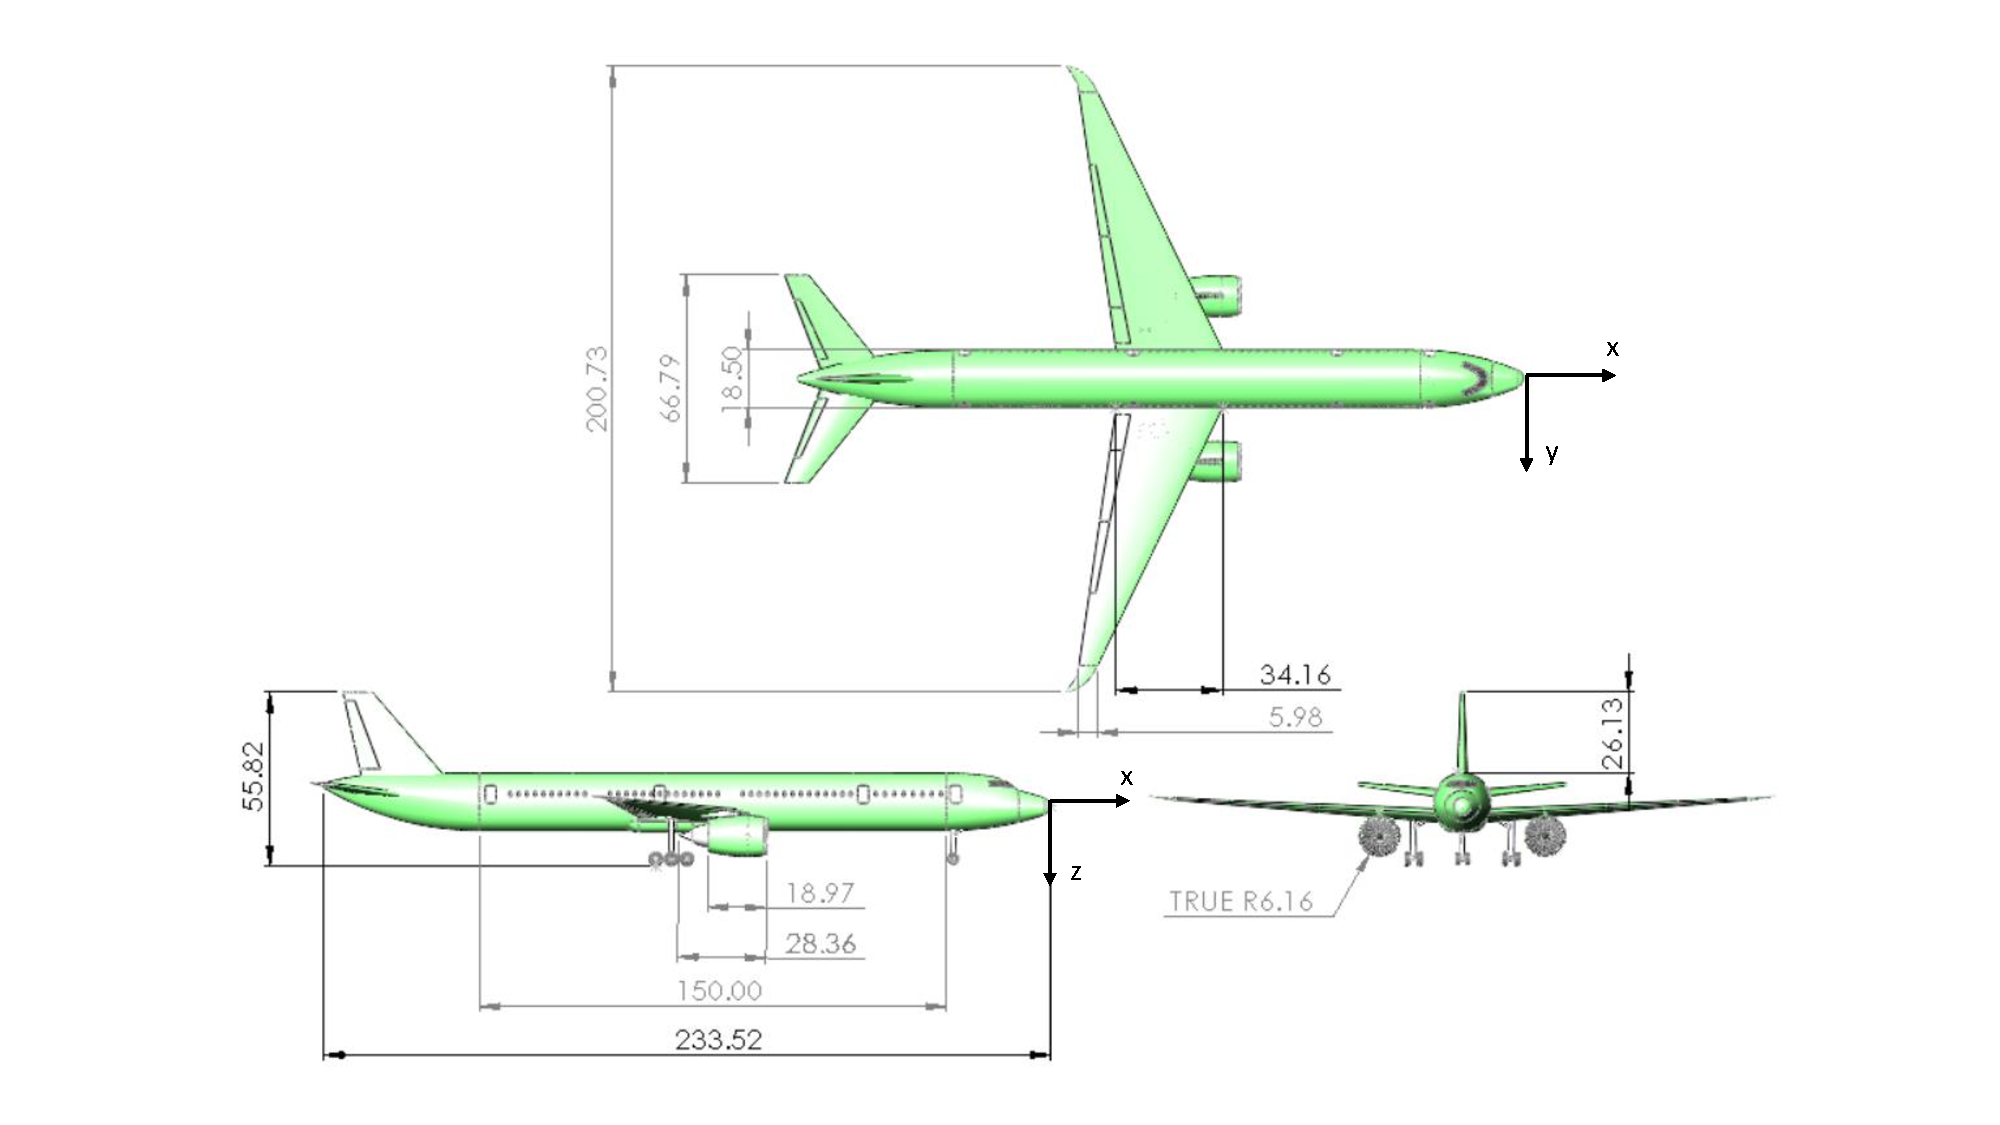
\includegraphics[width=\linewidth, angle =90 ]{Photos/3-view with coords_(4-27-20).pdf}
    \caption{3-View Drawing of SAM Mk 1 [ft]}
    \label{fig:threeview}
\end{figure}
\clearpage

\begin{figure}[!h]
    \centering
    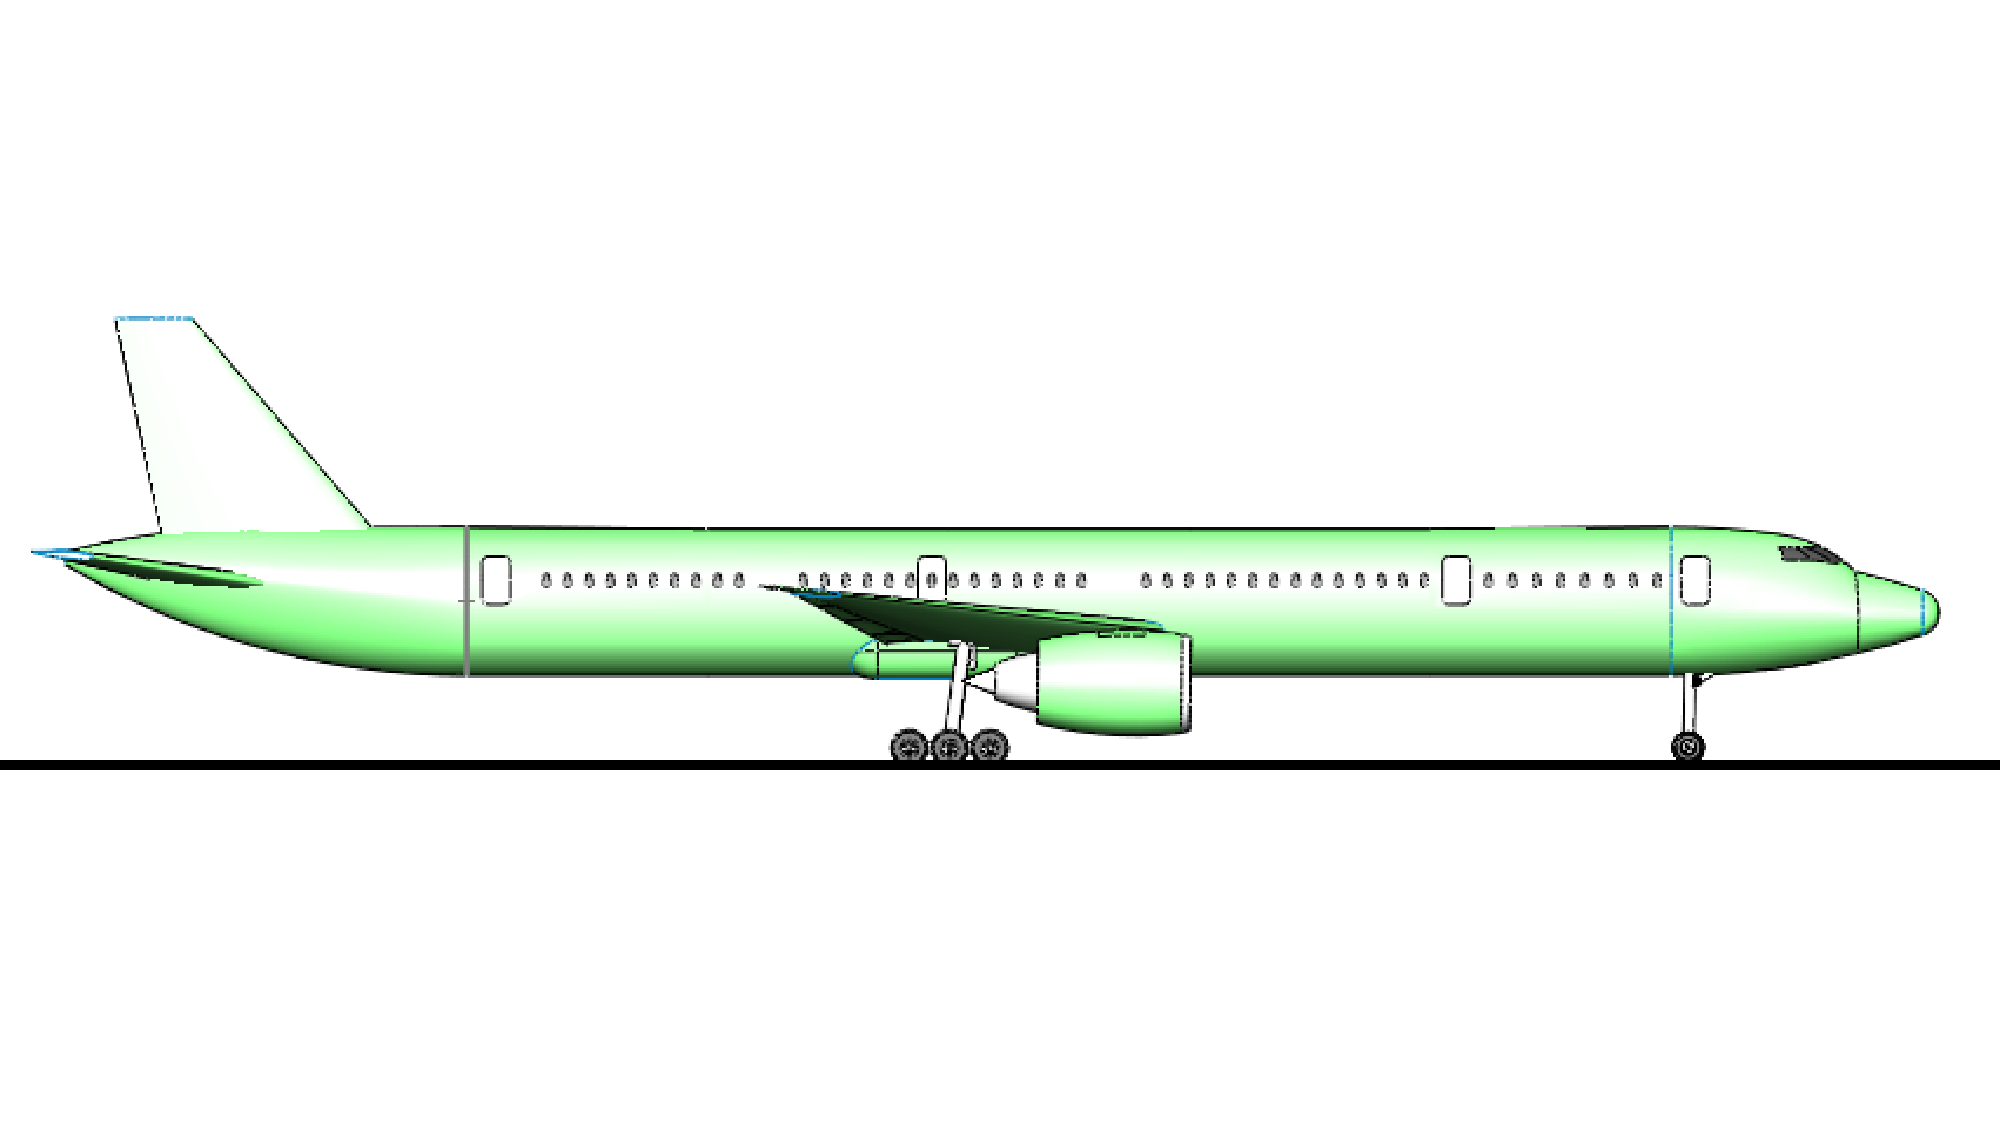
\includegraphics[width=1.0\textwidth]{Photos/Ground_Line.pdf}
    \caption{Side View of SAM Mk 1 with Ground Line}
    \label{grndline}
 \end{figure}

\subsection{Internal Configuration (\textit{JC})}
\label{section: internal config}
\subsubsection{Flight Deck Configuration}
The flight deck is configured for two pilots.  Adjustable seats enable ease of access to the control panels.  Pertaining to CFR $\S$ 25.775, the windscreens in the flight deck are inclined at $15\degree$ to the longitudinal axis.  An inside locking pop out emergency window is located on the port and starboard sides of the flight deck to provide the crew a quick emergency exit.

\clearpage 
\subsubsection{Seating Configuration (JC)}
The aircraft internal configuration is presented as two-class seating combining both business and economy seating accommodations.  Per AIAA RFP \cite{RFP} requirements, the aircraft is designed with 50 business-class and 350 economy-class seats to accommodate 400 total customers.  

\begin{table}[!h]
    \centering
    \caption{Seating Configuration}
    \begin{tabular}{|c|c||c|c|} \toprule
        \multicolumn{2}{c}{\textbf{Business Class}} & \multicolumn{2}{c}{\textbf{Economy Class}} \\ \hline
        Configuration (a) & 2 - 2 - 2 & Configuration (a) & 3 - 4 - 3 \\ \hline
        Row Count (a) & 8 & Row Count (a) & 28 \\ \hline
        Configuration (b) & 1 - 0 - 1 & Configuration (b) & 2 - 3 - 2 \\ \hline
        Row Count (b) & 1 & Row Count (b) & 10 \\ \hline
        Pitch & 36 [in] & Pitch & 32 [in] \\ \hline
        Width & 21 [in] & Width & 18 [in] \\ \bottomrule
    \end{tabular}
    \label{tab:seating}
\end{table}

Two different seating configurations are proposed for each class in Table \ref{tab:seating}, above.  The business class contains 8 rows with a 2 - 2 - 2 configuration to provide a spacious flight experience while making efficient use of the space provided.  The purpose of selecting a 2 - 2 - 2 style is to provide business passengers the opportunity to have aisle access.  The 1 - 0 - 1 row is provided to accommodate ADA passengers \cite{adaseating} and may be further customized by the client.  The economy class has two sections with a 3 - 4 - 3 and 2 - 3 - 2 configuration.  The 3 - 4 - 3 section provides high capacity seating while the 2 - 3 - 2 seating enables airliners to offer a highly competitive yet still profitable seating arrangement.

\begin{figure}[!h]
    \centering
    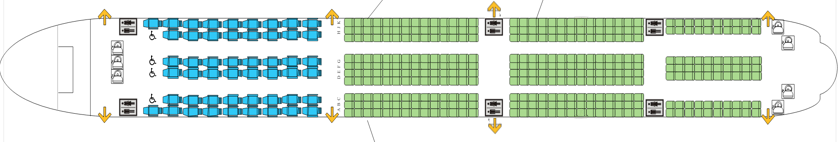
\includegraphics[width=\textwidth]{Photos/Config undimensioned.png}
    \caption{Internal Configuration}
    \label{fig:internalConfig}
\end{figure}

Crew seating can be oriented per customer request in the front and aft galleys and complies with 14 CFR \S 121.391(d).

\subsubsection{Galley Configuration}
SAM Mk 1 provides 2 galley locations, at the front and rear sections of the cabin.  This configuration optimizes crew capability of evenly servicing the two classes with minimal cross traffic.  By using the front entrance and aft sections of the cabin for galley and flight crew seating, there is 20 $ft^2$ of available space for airline partners to customize the galley sections to fit specific needs.
\clearpage 

\subsubsection{Lavatory Configuration}
SAM Mk 1 offers up to 6 lavatories in its 3,500 NM configuration to provide ease of access and mitigate aisle traffic.  Each lavatory is equipped with internal lighting, toilet facility, sanitation wipes, ash tray, emergency assistance button, and trash bin.  A sink and hand soap dispenser may be included per customer request; though sanitation wipes are provided as a weight saving measure.  The toilet facility uses negative pressure vacuum disposal system to vacate contents into a disposal tank stowed in the aft of the fuselage.\cite{toilet}  Lavatory doors are designed to lock from both the interior and the exterior for security.  Flight crew may be provided the key access to lock the lavatory doors from the exterior if a member on-board violates 14 CFR 91.11, 121.580, 135.120, 125.328, 49 USC 46318 \& 46504.  Configuration of lavatory may be modified to fit airline partner's needs.

\subsubsection{Door Configuration}
SAM Mk 1 provides 4 pairs of emergency doors, pursuant to 14 CFR \S25.807.  The front and aft loading doors are of Type A, defined by CFR \S25.813 and are 36 inches wide and 48 inches high.  These doors, when unlocked and activated, translate outwards and along the side of the fuselage.  The method of opening the emergency door is to allow maximum door clearance without requiring special boarding adapters from the jet bridge \cite{cfr}.  The two middle emergency exits are type I and are sized at 24 inches wide by 48 inches high.  The middle emergency doors are located by the lavatories and are spaced no farther than 60 feet from one another.  All four sets of the emergency doors include a Type II inflatable emergency slide/raft for passengers to evacuate \cite{slides}.

% \subsection{Certs that may apply}

% \texthl{25.775 - Windshields and windows - Is inclined 15 degrees or more to the longitudinal axis of the airplane}

% \texthl{25.813 - Emergency exit access - Shape of aisle in front of specific types of exits -> usually 36 inches wide  \\
% Each passageway leading to a Type A or Type B exit must be unobstructed and at least 36 inches wide. Passageways between individual passenger areas and those leading to Type I, Type II, or Type C emergency exits must be unobstructed and at least 20 inches wide. }




% \textcolor{red}{
% \begin{itemize}
%     \item Discuss external configuration alternatives considered and design choices made.
%     \begin{itemize}
%         \item \hl{Include a morphology wherein primary design alternatives are shown (via OpenVSP visual) and discussed (i.e. advantages/disadvantages) for different areas of consideration (i.e. wing placement, engine placement).}
%     \end{itemize}
%     \item Discuss selected aircraft configuration design (i.e. distinctions between variants, major features, design characteristics/objectives).
%     \begin{itemize}
%         \item \hl{Include a scaled 3-view drawing as comprehensive visuals that detail all major dimensions and parameters of the external configuration.}
%         \item \hl{Use a separate foldout for the 3-view.}
%         \item \hl{Show dimensions for: length, height, CG, and neutral point of entire aircraft; span, root and tip chord for wings, vertical tail, horizontal tail/stabilizer, flaps, ailerons, elevators, and rudder; length and diameter (width and height if non-circular) for fuselage and inlet(s); width and height of major door; height of landing gear.}
%         \item \hl{Show an overlay (dotted) of stowed landing gear (if applicable)}
%         \item \hl{Show ground lines.}
%     \end{itemize}
%     \item \hl{Discuss internal configuration design to meet objectives (i.e. customer appeal) and requirements (i.e. baggage capacity). !!!! for Josh to do}
%     \begin{itemize}
%         \item \hl{Include internal configuration drawing.}
%         \item \hl{Show dimensions for: cabin length, cabin width, cabin height, aisle width, passenger seats' length and width, width of door, and baggage compartment length and width.}
%     \end{itemize}
%     \item Include at least one trade study that uses quantitative or qualitative analysis to support design decisions made.
%     \item Discuss the landing gear philosophy.
%     \item 3-View drawing (VSP acceptable).
%     \item Discuss future work
%     \item AIAA: Complete geometric description, including dimensioned drawings, control surfaces sizes and hinge locations, and internal arrangement of the aircraft illustrating sufficient volume for all necessary components and systems to fulfill \#7 as seen \href{https://www.aiaa.org/docs/default-source/uploadedfiles/education-and-careers/university-students/design-competitions/undergraduate-team-aircraft-design-competition/undergraduate-aircraft-high-capacity-short-range-transport-aircraft.pdf?sfvrsn=b6081273_0}{here}: )
% \end{itemize}}